\documentclass{standalone}
\usepackage{tikz}
\usepackage{ctex,siunitx}
\setCJKmainfont{Noto Serif CJK SC}
\usepackage{tkz-euclide}
\usepackage{amsmath,upgreek}
\usetikzlibrary{patterns, calc,3d}
\usetikzlibrary {decorations.pathmorphing,decorations.pathreplacing,decorations.shapes}
\begin{document}
\small
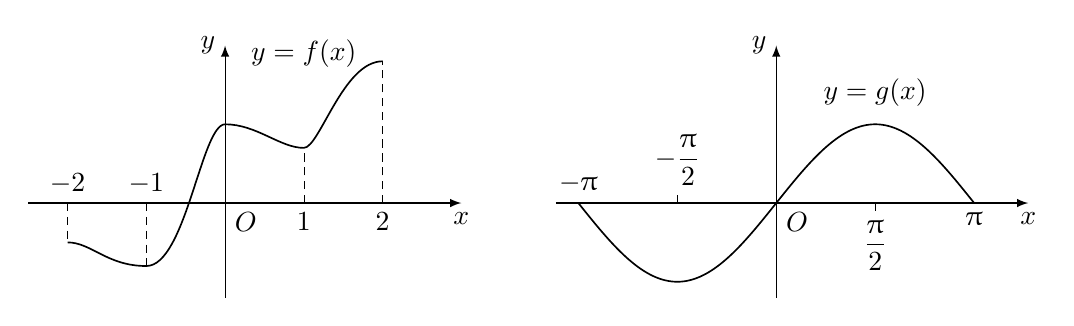
\begin{tikzpicture}[>=latex,scale=1.0]
  \begin{scope}
    \draw[->](-2.5,0)--(3,0)node[below]{$x$};
    \draw[->](0,-1.2)--(0,2.0)node[left]{$y$};
    \node at (0,0)[below right]{$O$};
    \draw[semithick](-2,-0.5)..controls(-1.7,-0.5)and(-1.5,-0.8)..
    (-1,-0.8)..controls(-0.5,-0.8)and(-0.3,1.0)..
    (0,1.0)..controls(0.4,1)and(0.7,0.7)..
    (1,0.7)..controls(1.2,0.7)and(1.5,1.8)..(2,1.8);
    \draw[very thin,densely dashed](-2,0)node[above]{$-2$}--(-2,-0.5);
    \draw[very thin,densely dashed](-1,0)node[above]{$-1$}--(-1,-0.8);
    \draw[very thin,densely dashed](1,0)node[below]{$1$}--(1,0.7);
    \draw[very thin,densely dashed](2,0)node[below]{$2$}--(2,1.8);
    \node at (1,1.9){$y=f(x)$};
  \end{scope}
  \begin{scope}[xshift=7cm,xscale=0.8]
    \draw[->](-3.5,0)--(4,0)node[below]{$x$};
    \draw[->](0,-1.2)--(0,2.0)node[left]{$y$};
    \node at (0,0)[below right]{$O$};
    \draw[semithick,samples=200,domain=-pi:pi]plot(\x,{sin(\x r)});
    \draw[very thin](-pi/2,0)--++(0,0.1)node[above]{$-\dfrac\uppi2$};
    \draw[very thin](pi/2,0)--++(0,-0.1)node[below]{$\dfrac\uppi2$};
    \node at (1.57,1.4){$y=g(x)$};
    \node at (-pi,0)[above]{$-\uppi$};
    \node at (pi,0)[below]{$\uppi$};
  \end{scope}
  
\end{tikzpicture}
\end{document}